\begin{figure}[t!]
\vspace{-10pt}
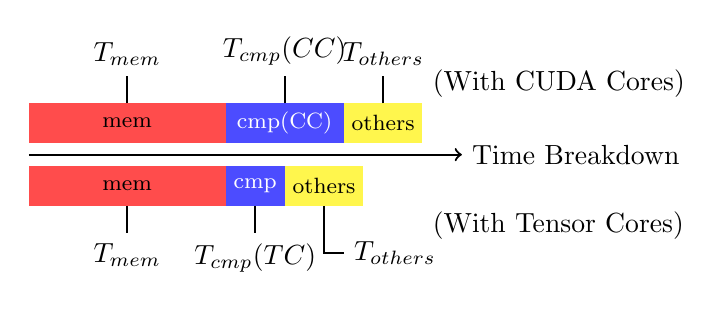
\begin{tikzpicture}[scale=0.5, every node/.style={scale=1}]
    % Timeline axis
    \draw[->, thick] (0,0) -- (11,0) node[right] {\textbf\footnotesize{Time Breakdown}};
    % Memory and Compute bars
    \fill[red!70] (0,0.3) rectangle (5,1.3) node[pos=.5,black] {\footnotesize{mem}};
    \fill[blue!70] (5,0.3) rectangle (8,1.3) node[pos=.5,white] {\footnotesize{cmp(CC)}};
    \fill[yellow!70] (8,0.3) rectangle (10,1.3) node[pos=.5,black] {\footnotesize{others}};

    \draw[thick] (2.5,1.3) -- (2.5,2) node[above] {$T_{\text{mem}}$};
    \draw[thick] (6.5,1.3) -- (6.5,2) node[above] {$T_{\text{cmp}}(CC)$};
    \draw[thick] (9,1.3) -- (9,2) node[above] {$T_{\text{others}}$};

    \draw[thick] (10,1.8) -- (10,1.8) node[right] {(With CUDA Cores)};


    \fill[red!70] (0,-0.3) rectangle (5,-1.3) node[pos=.5,black] {\footnotesize{mem}};
    \fill[blue!70] (5,-0.3) rectangle (6.5,-1.3) node[pos=.5,white] {\footnotesize{cmp}};
    \fill[yellow!70] (6.5,-0.3) rectangle (8.5,-1.3) node[pos=.5,black] {\footnotesize{others}};
    \draw[thick] (2.5,-1.3) -- (2.5,-2) node[below] {$T_{\text{mem}}$};
    \draw[thick] (5.75,-1.3) -- (5.75,-2) node[below] {$T_{\text{cmp}}(TC)$};
    \draw[thick] (7.5,-1.3) -- (7.5,-2.5) -- (8,-2.5) node[right] {$T_{\text{others}}$}; 

    \draw[thick] (10,-1.8) -- (10,-1.8) node[right] {(With Tensor Cores)};
\end{tikzpicture}
\vspace{-5pt}
\caption{Fully un-overlapped kernel time breakdown}\label{fig:breakout}
\end{figure}
